\section{Analysis}
\subsection{speedup}
\subsection{image errors verification}
Since we made several changes in the algorithm where we introduced some slight innaccuracies (for example using a fixed-point representation instead of floating point in the DSP), errors (deviations from the references implementation) are to be expected. Large errors are obvious to the eye, but this might be less obvious if the errors are only small. In this chapter we will detect and quantify these errors, to ensure that our implementation can still be considered correct.

\subsubsection{Error visualization}
Visualizing our errors is a fairly straightforward process. Because both images are constructed out of pixels with a grayscale value from 0 (black) to 255 (white), we can construct a new image by taking the difference between each pixel as a new pixel value. Note that this would give us a mapping where black indicates no difference, and brighter pixels indicating the difference. The inverse has more visual pop-out, so we subtract the difference from 255 to obtain our final pixel value. The implementation is described in Algorithm \ref{alg:imgdiff}. The result of this algorithm and a further comparison between the baseline and our implementation can be seen in figure~\ref{fig:imgdiff}.

An interesting observation is that we can clearly see that all the errors are in the lower area of the image, which is indeed the part that has been blurred by the DSP in a fixed point representation\footnote{This image has been produced with the load balancing of 35\% and 65\% for NEON and DSP respectively.}.

\begin{algorithm}[t]
    \caption{Constructing a image with the differences between two images}\label{alg:imgdiff}
    \begin{algorithmic}[1]
        \Procedure{DiffImage}{$A[N],B[N]$}  \Comment{Images A and B both have a size of N pixels}
        \State $C[N]\gets 0$
        \For{$i\gets 0, n-1$}
           \State $C[i]\gets 255 - |A[i] - B[i]|$   \Comment{Subtract the difference of A and B from 255}
        \EndFor
        \State \textbf{return} $C$
        \EndProcedure
    \end{algorithmic}
\end{algorithm}

\begin{figure}
    \centering
    \begin{subfigure}[b]{0.3\textwidth}
            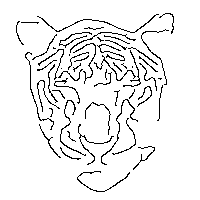
\includegraphics[width=\textwidth]{tiger_baseline}
            \caption{The baseline result}
            \label{fig:er_tiger_baseline}
    \end{subfigure}
    \begin{subfigure}[b]{0.3\textwidth}
            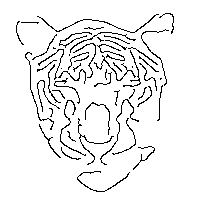
\includegraphics[width=\textwidth]{tiger_out}
            \caption{The optimized result}
            \label{fig:er_tiger_out}
    \end{subfigure}
    \begin{subfigure}[b]{0.3\textwidth}
            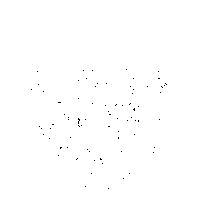
\includegraphics[width=\textwidth]{tiger_diff}
            \caption{The output of Algorithm~\ref{alg:imgdiff}}
            \label{fig:er_tiger_diff}
    \end{subfigure}
    \caption{Using the error visualization on an image of a tiger}
    \label{fig:imgdiff}
\end{figure}

\subsubsection{Error quantification}
In the visualization we can clearly spot some differences, but a further quantification would be nice as well. For this, we decided to use the \emph{Mean Squared Error}, as defined in equation~\ref{eq:mse}. This is an error-estimator giving us a quantification of the error rate. Since this number on it's own has little meaning, we decided to calculate the MSE rate of the baseline implementation and our optimized versions, both with respect to the original image and calculate the ratio between the difference and the reference error rate, to give us an error estimation. The results are given in table~\ref{tab:mse}. We find the final error ratio to be acceptable.

\begin{figure}[h]
    \begin{equation}
    MSE = \frac{1}{n} \sum_{i=0}^{n-1} (A[i] - B[i])^{2}
    \end{equation}
    \caption{Calculating the Mean Squared Error between images A and B, both n pixels large}
    \label{eq:mse}
\end{figure}

\begin{figure}[h!]
    \centering
    \begin{tabular}{l | l l l l}
    Image   & Reference MSE & Optimized MSE     & Difference    & Ratio     \\
    \hline
    Square  & 10643.083984  & 10906.207031      & 263.123047    & 0.024722  \\
    Tiger   & 46683.480469  & 46678.214844      & 5.265625      & 0.000113  \\
    Klomp   & 20535.517578  & 20509.070312      & 26.447266     & 0.001288
    \end{tabular}
    \caption{The calculated mean squared error}
    \label{tab:mse}
\end{figure}
